\chapter{Kaldi学习笔记}
\section{kaldi中的数据扰动}
kaldi程序中对原始数据进行扰动以达到数据增强的效果,一般是在单音素对齐,三音素对齐之后,在生成ivector的时候进行扰动处理,扰动有两种方式:速度扰动和音量扰动。如果存在segment文件的话,那么对应的起始和终止时间点会存在segment文件中,提取特征时会根据这个segment中存储的时间节点进行操作;如果不存在的话,相当于整段wav音频都是有效的,那么起始时间点和wav文件相同。扰动也会根据segment文件的有无进行对应的操作。

\subsection{速度扰动}

速度扰动一般是对音频进行加速和减速,根据Povey大佬的论文\href{https://www.danielpovey.com/files/2015_interspeech_augmentation.pdf}{《Audio Augmentation for Speech Recognition》}中的第二部分Audio Perturbation,对mel频谱进行一个偏移就能得到类似加速和减速的效果。首先定义一个扰动因子$\alpha$,假定segment中某一段音频的起始时间和终止时间为$t_1$和$t_2$,那么新的音频起始时间和终止时间计算方式如公式\ref{eqn:sp}。
\begin{align}
\label{eqn:sp}
\begin{split}
  t_{1}' = \frac{t_1}{\alpha} \\
  t_{2}' = \frac{t_2}{\alpha}
\end{split}
\end{align}

kaldi一般取$\alpha$为$0.9$和$1.1$以达到加速和减速的目的。得到了segment文件之后,在wav.scp文件中存储原始音频的位置,加速后音频sox指令和减速后音频sox指令。其详细的脚本指令见代码 utils/data/perturb\_data\_dir\_speed.sh 第74行。最终重新提取特征存于代码根目录下mfcc\_pertubed文件夹中。由于速度扰动对音频时间轴有改动,因此此时需要对音频进行重新对齐的操作。

\subsection{音量扰动}
音量扰动一般是对音频进行增大音量和减小音量。音量增加或者减小的幅度默认取$[0.125, 2]$之间的正态分布值。使用sox工具中的"sox - -vol #volume"来进行实际操作。其详细的脚本指令见代码 utils/data/perturb\_data\_dir\_volume.sh 第71行,其sox操作见代码 utils/data/internal/perturb\_volume.py。其重新提取的特征位于代码根目录下mfcc\_hires 文件夹中。此时由于仅仅对音频进行音量大小的扰动,并没有对时间维度进行操作,因此无需再进行一遍对齐操作,其标签对齐直接采用上一步即速度扰动后生成的对齐结果。此时重新提取特征时,MFCC特征的维度是40d。其原因是40d的MFCC和40d的Fbank维度相同,保存的信息量相似,同时MFCC由于其相关性较弱(DCT去相关),所以能更好的压缩特征,因此Kaldi一般都是采用40d的MFCC作为神经网络的输入特征(见kaldi的各个egs里conf下mfcc\_hires.conf)。
\begin{quotation}
"Config for high-resolution MFCC features, intended for neural network training. Note: we keep all cepstra, so it has the same info as filterbank features, but MFCC is more easily compressible (because less correlated) which is why we prefer this method. "
\end{quotation}

\section{kaldi中的UBM}

\href{http://citeseerx.ist.psu.edu/viewdoc/download?doi=10.1.1.117.338&rep=rep1&type=pdf}{通用背景模型UBM}(Universal Background Model)

\section{kaldi通过lattice输出语音对齐音素和词}

我们通过解码之后得到一堆的 lat.*.gz 文件,这些文件是lattice对齐后生成的对齐文件,其为压缩格式,所以首先通过 gunzip 指令对齐解压,我们以 lat.1.gz 为例来讲这一节的知识点。
\begin{lstlisting}[language=shell, numbers=left, 
         numberstyle=\tiny,keywordstyle=\color{blue!70},
         commentstyle=\color{red!50!green!50!blue!50},frame=shadowbox,
         rulesepcolor=\color{red!20!green!20!blue!20},basicstyle=\ttfamily]
gunzip exp/chain/tdnn7q_sp_online/decode_data_tgsmall/lat.1.gz
\end{lstlisting}

这样会在 exp/chain/tdnn7q\_sp\_online/decode\_data\_tgsmall/ 下生成一个 lat.1 文件,原先的 lat.1.gz 消失不见了…… lat.1 文件是二进制的格式,其由指令 online2-wav-nnet3-latgen-fatser 生成。

\section{kaldi中的数据准备}
\subsection{音频、文本、说话人准备}

\subsetion{准备词典}
词典的作用是将词映射成音素,不论是基于HMM-GMM的对齐,还是HMM-DNN的声学模型训练,其建模单元为音素,但是在实际交流中,我们看到的都是词或者词组成的句子,因此我们需要这么一个文件,在对齐或者训练声学的时候,将词映射成发音;在解码的时候我们看到的是词而不是音素,因此需要训练语言模型将音素转换成最有可能的词。因此,词典是非常非常重要的。

首先 lexicon.txt 的格式是 {\bf "<word>\qquad<pronunciation>"}。对应的"<pronounciation>"就是词的音素。表\ref{tab:lexicon-format}分别展示了中英文的lexicon.txt的示例。
\begin{table}[h]
\centering
\caption{中英文word和对应pronounciation示例}
   \begin{tabular*}{1\textwidth}{@{\extracolsep{\fill}}cc}
   \toprule
    {\bf Word} & {\bf Pronouciation} \\
   \midrule
   七叶树   & qi iH iH yi ehH ehL shu uH uL \\
   episode & EH1 P IH0 S OW2 D  \\
   \bottomrule
   \end{tabular*}
 \label{tab:lexicon-format}
\end{table}

在准备词典的时候,其对应的路径为{\bf data/local/lm},其文本内容类似于图\ref{fig:lexicon-fig}。词和发音之间以Tab隔开,音素之间以空格隔开。
\begin{figure}[!ht]
  \centering
  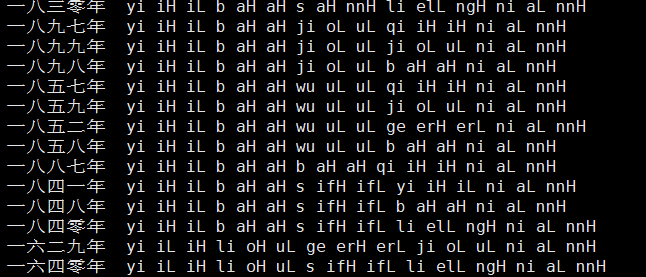
\includegraphics[width=0.55\textwidth]{lexicon-fig}
  \caption{lexicon.txt中存储格式}
\label{fig:lexicon-fig}
\end{figure}

另外一个很重要的文件是vocab.txt,其路径为{\bf data/local/lm/vocab.txt}。其存储了待建模的数据库中包含的所有的词。如果是中文的话,就需要对中文语句进行分词,如果对应的数据库已经分好了词,那么


\section{kaldi中的决策树}
\label{sec:kaldi-dt}


\section{kaldi错误及解决办法集锦}
\begin{enumerate}
  \item ERROR: FstHeader::Read: Bad FST header: -:出现的原因是Memory不够,语言模型太大了。构图的时候,在终端输入top指令,再摁个E,就可以很清晰的看到随着构图的进行,Memory逐渐被吃掉……
  log如下:
  \begin{lstlisting}[language=shell, numbers=left, 
         numberstyle=\tiny,keywordstyle=\color{blue!70},
         commentstyle=\color{red!50!green!50!blue!50},frame=shadowbox,
         rulesepcolor=\color{red!20!green!20!blue!20},basicstyle=\ttfamily]
fstminimizeencoded 
fstdeterminizestar --use-log=true 
fsttablecompose /data2/src/tmp/big-lm/lang_pp_test_tgsmall/L_disambig.fst /data2/src/tmp/big-lm/lang_pp_test_tgsmall/G.fst 
fstpushspecial 
ERROR: FstHeader::Read: Bad FST header: -
ERROR (fstdeterminizestar[5.5]:ReadFstKaldi():kaldi-fst-io.cc:35) Reading FST: error reading FST header from standard input

[ Stack-Trace: ]
kaldi::MessageLogger::LogMessage() const
kaldi::MessageLogger::LogAndThrow::operator=(kaldi::MessageLogger const&)
fst::ReadFstKaldi(std::string)
main
__libc_start_main
fstdeterminizestar() [0x425209]

kaldi::KaldiFatalErrorERROR: FstHeader::Read: Bad FST header: -
ERROR (fstminimizeencoded[5.5]:ReadFstKaldi():kaldi-fst-io.cc:35) Reading FST: error reading FST header from standard input

[ Stack-Trace: ]
kaldi::MessageLogger::LogMessage() const
kaldi::MessageLogger::LogAndThrow::operator=(kaldi::MessageLogger const&)
fst::ReadFstKaldi(std::string)
main
__libc_start_main
fstminimizeencoded() [0x413559]

kaldi::KaldiFatalErrorERROR: FstHeader::Read: Bad FST header: -
ERROR (fstpushspecial[5.5]:ReadFstKaldi():kaldi-fst-io.cc:35) Reading FST: error reading FST header from standard input

[ Stack-Trace: ]
kaldi::MessageLogger::LogMessage() const
kaldi::MessageLogger::LogAndThrow::operator=(kaldi::MessageLogger const&)
fst::ReadFstKaldi(std::string)
main
__libc_start_main
fstpushspecial() [0x401b99]
  \end{lstlisting}
  那么我们怎么来使用大的语言模型呢?可以先用小的语言模型参与解码,然后生成对应的lattice,再使用rescoring的方法利用大的语言模型来进行重新估计,解决步骤如下:
  \begin{enumerate}
      \item 使用 \textcolor{green}{utils/format\_lm.sh} 生成小语言模型的G.fst;
      \item 使用 \textcolor{green}{utils/format\_lm.sh} 生成大语言模型的G.fst;
      \item 使用 \textcolor{green}{utils/mkgraph.sh} 来逐步构图,生成HCLG.fst;
      \item 使用 \textcolor{green}{steps/online/nnet3/prepare\_online\_decoding.sh}来准备在线解码;
      \item 使用 \textcolor{green}{steps/online/nnet3/decode.sh}来进行在线解码生成lattice;
      \item 使用 \textcolor{green}{steps/lmrescore.sh} 来进行rescoring。切记{\bf 如果是chain model,在运行这条指令时要加上 "--self-loop-scale 1.0"}。
  \end{enumerate}
\item ……

\end{enumerate}

\section{OpenFst}
